\documentclass[12pt,a4paper]{article}

\usepackage[a4paper,text={16.5cm,25.2cm},centering]{geometry}
\usepackage{lmodern}
\usepackage{amssymb,amsmath}
\usepackage{bm}
\usepackage{graphicx}
\usepackage{microtype}
\usepackage{hyperref}
\setlength{\parindent}{0pt}
\setlength{\parskip}{1.2ex}

\hypersetup
       {   pdfauthor = { Kevin Corcoran },
           pdftitle={ HW \#3 Computational },
           colorlinks=TRUE,
           linkcolor=black,
           citecolor=blue,
           urlcolor=blue
       }

\title{ HW \#3 Computational }

\author{ Kevin Corcoran }


\usepackage{upquote}
\usepackage{listings}
\usepackage{xcolor}
\lstset{
    basicstyle=\ttfamily\footnotesize,
    upquote=true,
    breaklines=true,
    breakindent=0pt,
    keepspaces=true,
    showspaces=false,
    columns=fullflexible,
    showtabs=false,
    showstringspaces=false,
    escapeinside={(*@}{@*)},
    extendedchars=true,
}
\newcommand{\HLJLt}[1]{#1}
\newcommand{\HLJLw}[1]{#1}
\newcommand{\HLJLe}[1]{#1}
\newcommand{\HLJLeB}[1]{#1}
\newcommand{\HLJLo}[1]{#1}
\newcommand{\HLJLk}[1]{\textcolor[RGB]{148,91,176}{\textbf{#1}}}
\newcommand{\HLJLkc}[1]{\textcolor[RGB]{59,151,46}{\textit{#1}}}
\newcommand{\HLJLkd}[1]{\textcolor[RGB]{214,102,97}{\textit{#1}}}
\newcommand{\HLJLkn}[1]{\textcolor[RGB]{148,91,176}{\textbf{#1}}}
\newcommand{\HLJLkp}[1]{\textcolor[RGB]{148,91,176}{\textbf{#1}}}
\newcommand{\HLJLkr}[1]{\textcolor[RGB]{148,91,176}{\textbf{#1}}}
\newcommand{\HLJLkt}[1]{\textcolor[RGB]{148,91,176}{\textbf{#1}}}
\newcommand{\HLJLn}[1]{#1}
\newcommand{\HLJLna}[1]{#1}
\newcommand{\HLJLnb}[1]{#1}
\newcommand{\HLJLnbp}[1]{#1}
\newcommand{\HLJLnc}[1]{#1}
\newcommand{\HLJLncB}[1]{#1}
\newcommand{\HLJLnd}[1]{\textcolor[RGB]{214,102,97}{#1}}
\newcommand{\HLJLne}[1]{#1}
\newcommand{\HLJLneB}[1]{#1}
\newcommand{\HLJLnf}[1]{\textcolor[RGB]{66,102,213}{#1}}
\newcommand{\HLJLnfm}[1]{\textcolor[RGB]{66,102,213}{#1}}
\newcommand{\HLJLnp}[1]{#1}
\newcommand{\HLJLnl}[1]{#1}
\newcommand{\HLJLnn}[1]{#1}
\newcommand{\HLJLno}[1]{#1}
\newcommand{\HLJLnt}[1]{#1}
\newcommand{\HLJLnv}[1]{#1}
\newcommand{\HLJLnvc}[1]{#1}
\newcommand{\HLJLnvg}[1]{#1}
\newcommand{\HLJLnvi}[1]{#1}
\newcommand{\HLJLnvm}[1]{#1}
\newcommand{\HLJLl}[1]{#1}
\newcommand{\HLJLld}[1]{\textcolor[RGB]{148,91,176}{\textit{#1}}}
\newcommand{\HLJLs}[1]{\textcolor[RGB]{201,61,57}{#1}}
\newcommand{\HLJLsa}[1]{\textcolor[RGB]{201,61,57}{#1}}
\newcommand{\HLJLsb}[1]{\textcolor[RGB]{201,61,57}{#1}}
\newcommand{\HLJLsc}[1]{\textcolor[RGB]{201,61,57}{#1}}
\newcommand{\HLJLsd}[1]{\textcolor[RGB]{201,61,57}{#1}}
\newcommand{\HLJLsdB}[1]{\textcolor[RGB]{201,61,57}{#1}}
\newcommand{\HLJLsdC}[1]{\textcolor[RGB]{201,61,57}{#1}}
\newcommand{\HLJLse}[1]{\textcolor[RGB]{59,151,46}{#1}}
\newcommand{\HLJLsh}[1]{\textcolor[RGB]{201,61,57}{#1}}
\newcommand{\HLJLsi}[1]{#1}
\newcommand{\HLJLso}[1]{\textcolor[RGB]{201,61,57}{#1}}
\newcommand{\HLJLsr}[1]{\textcolor[RGB]{201,61,57}{#1}}
\newcommand{\HLJLss}[1]{\textcolor[RGB]{201,61,57}{#1}}
\newcommand{\HLJLssB}[1]{\textcolor[RGB]{201,61,57}{#1}}
\newcommand{\HLJLnB}[1]{\textcolor[RGB]{59,151,46}{#1}}
\newcommand{\HLJLnbB}[1]{\textcolor[RGB]{59,151,46}{#1}}
\newcommand{\HLJLnfB}[1]{\textcolor[RGB]{59,151,46}{#1}}
\newcommand{\HLJLnh}[1]{\textcolor[RGB]{59,151,46}{#1}}
\newcommand{\HLJLni}[1]{\textcolor[RGB]{59,151,46}{#1}}
\newcommand{\HLJLnil}[1]{\textcolor[RGB]{59,151,46}{#1}}
\newcommand{\HLJLnoB}[1]{\textcolor[RGB]{59,151,46}{#1}}
\newcommand{\HLJLoB}[1]{\textcolor[RGB]{102,102,102}{\textbf{#1}}}
\newcommand{\HLJLow}[1]{\textcolor[RGB]{102,102,102}{\textbf{#1}}}
\newcommand{\HLJLp}[1]{#1}
\newcommand{\HLJLc}[1]{\textcolor[RGB]{153,153,119}{\textit{#1}}}
\newcommand{\HLJLch}[1]{\textcolor[RGB]{153,153,119}{\textit{#1}}}
\newcommand{\HLJLcm}[1]{\textcolor[RGB]{153,153,119}{\textit{#1}}}
\newcommand{\HLJLcp}[1]{\textcolor[RGB]{153,153,119}{\textit{#1}}}
\newcommand{\HLJLcpB}[1]{\textcolor[RGB]{153,153,119}{\textit{#1}}}
\newcommand{\HLJLcs}[1]{\textcolor[RGB]{153,153,119}{\textit{#1}}}
\newcommand{\HLJLcsB}[1]{\textcolor[RGB]{153,153,119}{\textit{#1}}}
\newcommand{\HLJLg}[1]{#1}
\newcommand{\HLJLgd}[1]{#1}
\newcommand{\HLJLge}[1]{#1}
\newcommand{\HLJLgeB}[1]{#1}
\newcommand{\HLJLgh}[1]{#1}
\newcommand{\HLJLgi}[1]{#1}
\newcommand{\HLJLgo}[1]{#1}
\newcommand{\HLJLgp}[1]{#1}
\newcommand{\HLJLgs}[1]{#1}
\newcommand{\HLJLgsB}[1]{#1}
\newcommand{\HLJLgt}[1]{#1}


\begin{document}

\maketitle

\section{Including required packages}

\begin{lstlisting}
(*@\HLJLk{using}@*) (*@\HLJLn{Plots}@*)
(*@\HLJLk{using}@*) (*@\HLJLn{LaTeXStrings}@*)
(*@\HLJLnf{theme}@*)(*@\HLJLp{(}@*)(*@\HLJLsc{:mute}@*)(*@\HLJLp{)}@*)

(*@\HLJLk{using}@*) (*@\HLJLn{Pkg}@*)
(*@\HLJLn{Pkg}@*)(*@\HLJLoB{.}@*)(*@\HLJLnf{activate}@*)(*@\HLJLp{(}@*)(*@\HLJLs{"{}RAS"{}}@*)(*@\HLJLp{)}@*)
(*@\HLJLnf{include}@*)(*@\HLJLp{(}@*)(*@\HLJLs{"{}code/RAS.jl"{}}@*)(*@\HLJLp{)}@*) (*@\HLJLcs{{\#}}@*) (*@\HLJLcs{Makes}@*) (*@\HLJLcs{sure}@*) (*@\HLJLcs{the}@*) (*@\HLJLcs{module}@*) (*@\HLJLcs{is}@*) (*@\HLJLcs{run}@*) (*@\HLJLcs{before}@*) (*@\HLJLcs{using}@*) (*@\HLJLcs{it}@*)
(*@\HLJLk{using}@*) (*@\HLJLoB{.}@*)(*@\HLJLn{RAS}@*)(*@\HLJLoB{:}@*) (*@\HLJLn{RAS{\_}stabf}@*)(*@\HLJLp{,}@*) (*@\HLJLn{RASrk}@*)

(*@\HLJLn{Pkg}@*)(*@\HLJLoB{.}@*)(*@\HLJLnf{activate}@*)(*@\HLJLp{(}@*)(*@\HLJLs{"{}DiffyQ"{}}@*)(*@\HLJLp{)}@*)
(*@\HLJLnf{include}@*)(*@\HLJLp{(}@*)(*@\HLJLs{"{}code/DiffyQ.jl"{}}@*)(*@\HLJLp{)}@*) (*@\HLJLcs{{\#}}@*) (*@\HLJLcs{Makes}@*) (*@\HLJLcs{sure}@*) (*@\HLJLcs{the}@*) (*@\HLJLcs{module}@*) (*@\HLJLcs{is}@*) (*@\HLJLcs{run}@*) (*@\HLJLcs{before}@*) (*@\HLJLcs{using}@*) (*@\HLJLcs{it}@*)
(*@\HLJLk{using}@*) (*@\HLJLoB{.}@*)(*@\HLJLn{DiffyQ}@*)(*@\HLJLoB{:}@*) (*@\HLJLn{s2{\_}DIRK}@*)(*@\HLJLp{,}@*) (*@\HLJLn{BackwardEuler{\_}n}@*)
\end{lstlisting}


\section{Problem 4: Plot Region of Absolute Stability}
Note that "light" color is the region of stability


\begin{lstlisting}
(*@\HLJLcs{{\#}}@*) (*@\HLJLcs{stability}@*) (*@\HLJLcs{function}@*) (*@\HLJLcs{for}@*) (*@\HLJLcs{Heun{\textquotesingle}s}@*)
(*@\HLJLnf{\ensuremath{\Phi}}@*)(*@\HLJLp{(}@*)(*@\HLJLn{z}@*)(*@\HLJLp{)}@*) (*@\HLJLoB{=}@*) (*@\HLJLnfB{1.0}@*) (*@\HLJLoB{+}@*) (*@\HLJLn{z}@*) (*@\HLJLoB{+}@*) (*@\HLJLn{z}@*)(*@\HLJLoB{{\textasciicircum}}@*)(*@\HLJLni{2}@*)
(*@\HLJLn{xs}@*)(*@\HLJLp{,}@*) (*@\HLJLn{Z}@*) (*@\HLJLoB{=}@*) (*@\HLJLnf{RAS{\_}stabf}@*)(*@\HLJLp{(}@*)(*@\HLJLn{\ensuremath{\Phi}}@*)(*@\HLJLp{)}@*)

(*@\HLJLnf{contourf}@*)(*@\HLJLp{(}@*)(*@\HLJLn{xs}@*)(*@\HLJLp{,}@*) (*@\HLJLn{xs}@*)(*@\HLJLp{,}@*) (*@\HLJLn{Z}@*)(*@\HLJLp{,}@*) (*@\HLJLn{levels}@*) (*@\HLJLoB{=}@*) (*@\HLJLni{1}@*)(*@\HLJLp{)}@*)
\end{lstlisting}

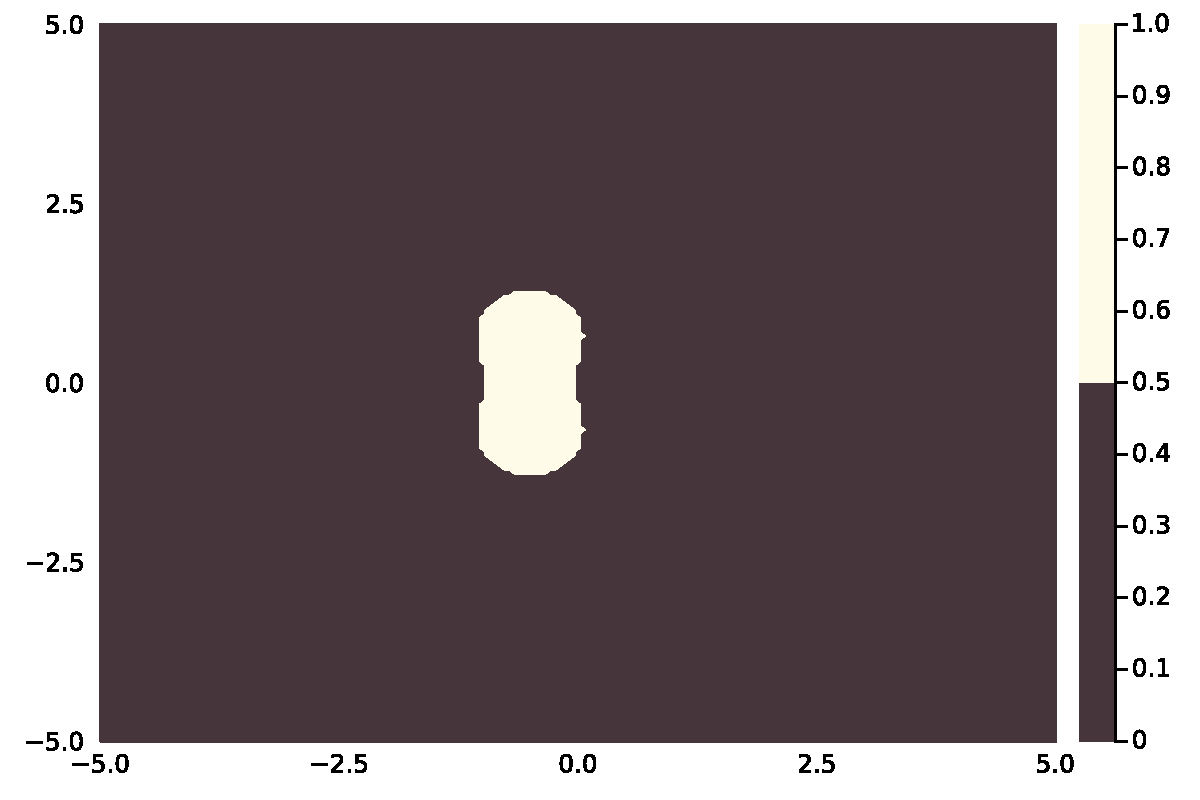
\includegraphics[width=\linewidth]{figures/ass_3_report_2_1.pdf}

\begin{lstlisting}
(*@\HLJLcs{{\#}}@*) (*@\HLJLcs{RK4}@*)
(*@\HLJLn{A}@*) (*@\HLJLoB{=}@*) (*@\HLJLp{[}@*)(*@\HLJLni{0}@*) (*@\HLJLni{0}@*) (*@\HLJLni{0}@*) (*@\HLJLni{0}@*)
    (*@\HLJLni{1}@*)(*@\HLJLoB{/}@*)(*@\HLJLni{2}@*) (*@\HLJLni{0}@*) (*@\HLJLni{0}@*) (*@\HLJLni{0}@*)
    (*@\HLJLni{0}@*) (*@\HLJLni{1}@*)(*@\HLJLoB{/}@*)(*@\HLJLni{2}@*) (*@\HLJLni{0}@*) (*@\HLJLni{0}@*)
    (*@\HLJLni{0}@*) (*@\HLJLni{0}@*) (*@\HLJLni{1}@*) (*@\HLJLni{0}@*)(*@\HLJLp{]}@*)
(*@\HLJLn{b}@*) (*@\HLJLoB{=}@*) (*@\HLJLp{[}@*)(*@\HLJLni{1}@*)(*@\HLJLoB{/}@*)(*@\HLJLni{6}@*)(*@\HLJLp{,}@*) (*@\HLJLni{1}@*)(*@\HLJLoB{/}@*)(*@\HLJLni{3}@*)(*@\HLJLp{,}@*) (*@\HLJLni{1}@*)(*@\HLJLoB{/}@*)(*@\HLJLni{3}@*)(*@\HLJLp{,}@*) (*@\HLJLni{1}@*)(*@\HLJLoB{/}@*)(*@\HLJLni{6}@*)(*@\HLJLp{]}@*)

(*@\HLJLn{xs}@*)(*@\HLJLp{,}@*) (*@\HLJLn{Z}@*) (*@\HLJLoB{=}@*) (*@\HLJLnf{RASrk}@*)(*@\HLJLp{(}@*)(*@\HLJLn{A}@*)(*@\HLJLp{,}@*)(*@\HLJLn{b}@*)(*@\HLJLp{)}@*)
(*@\HLJLcs{{\#}}@*) (*@\HLJLcs{plotly()}@*)
(*@\HLJLnf{contourf}@*)(*@\HLJLp{(}@*)(*@\HLJLn{xs}@*)(*@\HLJLp{,}@*)(*@\HLJLn{xs}@*)(*@\HLJLp{,}@*)(*@\HLJLn{Z}@*)(*@\HLJLp{,}@*) (*@\HLJLn{levels}@*) (*@\HLJLoB{=}@*) (*@\HLJLni{1}@*)(*@\HLJLp{)}@*)
\end{lstlisting}

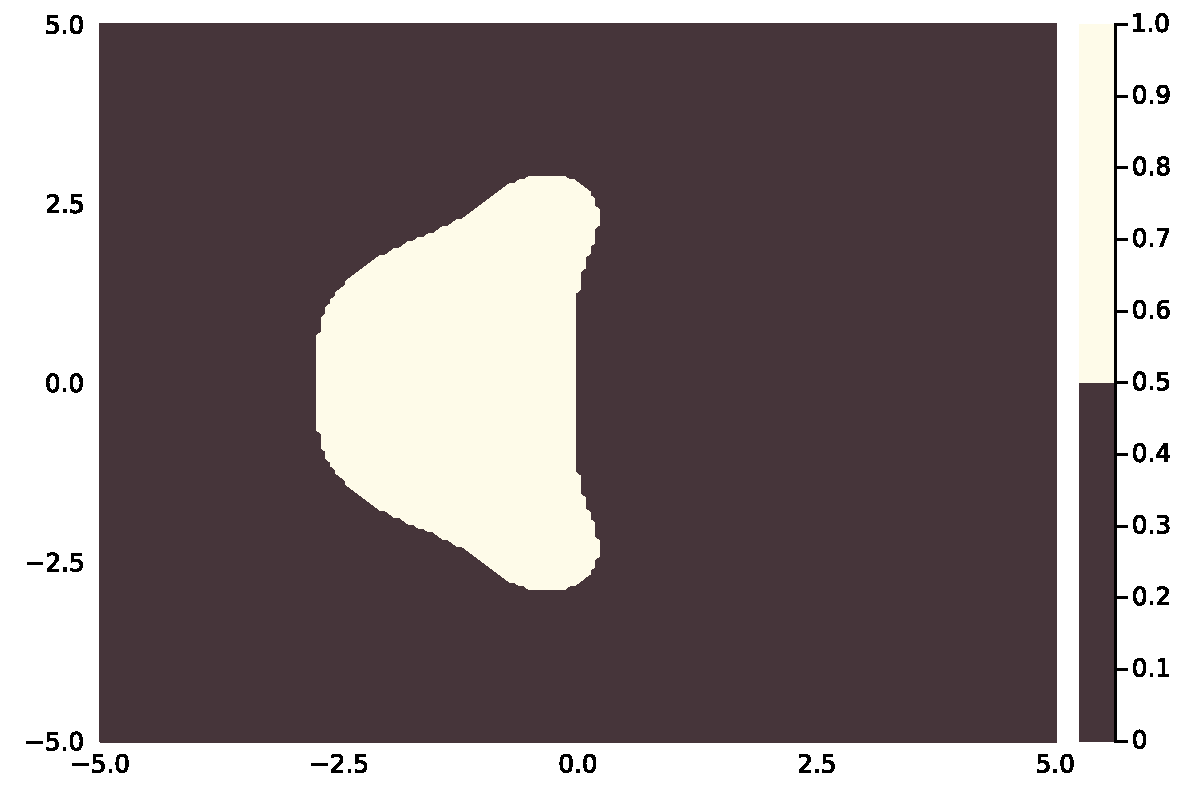
\includegraphics[width=\linewidth]{figures/ass_3_report_3_1.pdf}

\begin{lstlisting}
(*@\HLJLcs{{\#}}@*) (*@\HLJLcs{2s-DIRK}@*)
(*@\HLJLn{\ensuremath{\alpha}}@*) (*@\HLJLoB{=}@*) (*@\HLJLni{1}@*)(*@\HLJLoB{-}@*)(*@\HLJLni{1}@*)(*@\HLJLoB{/}@*)(*@\HLJLnf{sqrt}@*)(*@\HLJLp{(}@*)(*@\HLJLni{2}@*)(*@\HLJLp{)}@*)
(*@\HLJLn{A}@*) (*@\HLJLoB{=}@*) (*@\HLJLp{[}@*)(*@\HLJLn{\ensuremath{\alpha}}@*) (*@\HLJLni{0}@*)
    (*@\HLJLni{1}@*)(*@\HLJLoB{-}@*)(*@\HLJLn{\ensuremath{\alpha}}@*) (*@\HLJLn{\ensuremath{\alpha}}@*)(*@\HLJLp{]}@*)
(*@\HLJLn{b}@*) (*@\HLJLoB{=}@*) (*@\HLJLp{[}@*)(*@\HLJLni{1}@*)(*@\HLJLoB{-}@*)(*@\HLJLn{\ensuremath{\alpha}}@*)(*@\HLJLp{,}@*) (*@\HLJLn{\ensuremath{\alpha}}@*)(*@\HLJLp{]}@*)

(*@\HLJLn{xs}@*)(*@\HLJLp{,}@*) (*@\HLJLn{Z}@*) (*@\HLJLoB{=}@*) (*@\HLJLnf{RASrk}@*)(*@\HLJLp{(}@*)(*@\HLJLn{A}@*)(*@\HLJLp{,}@*)(*@\HLJLn{b}@*)(*@\HLJLp{)}@*)
(*@\HLJLnf{contourf}@*)(*@\HLJLp{(}@*)(*@\HLJLn{xs}@*)(*@\HLJLp{,}@*)(*@\HLJLn{xs}@*)(*@\HLJLp{,}@*)(*@\HLJLn{Z}@*)(*@\HLJLp{,}@*) (*@\HLJLn{levels}@*) (*@\HLJLoB{=}@*) (*@\HLJLni{1}@*)(*@\HLJLp{)}@*)
\end{lstlisting}

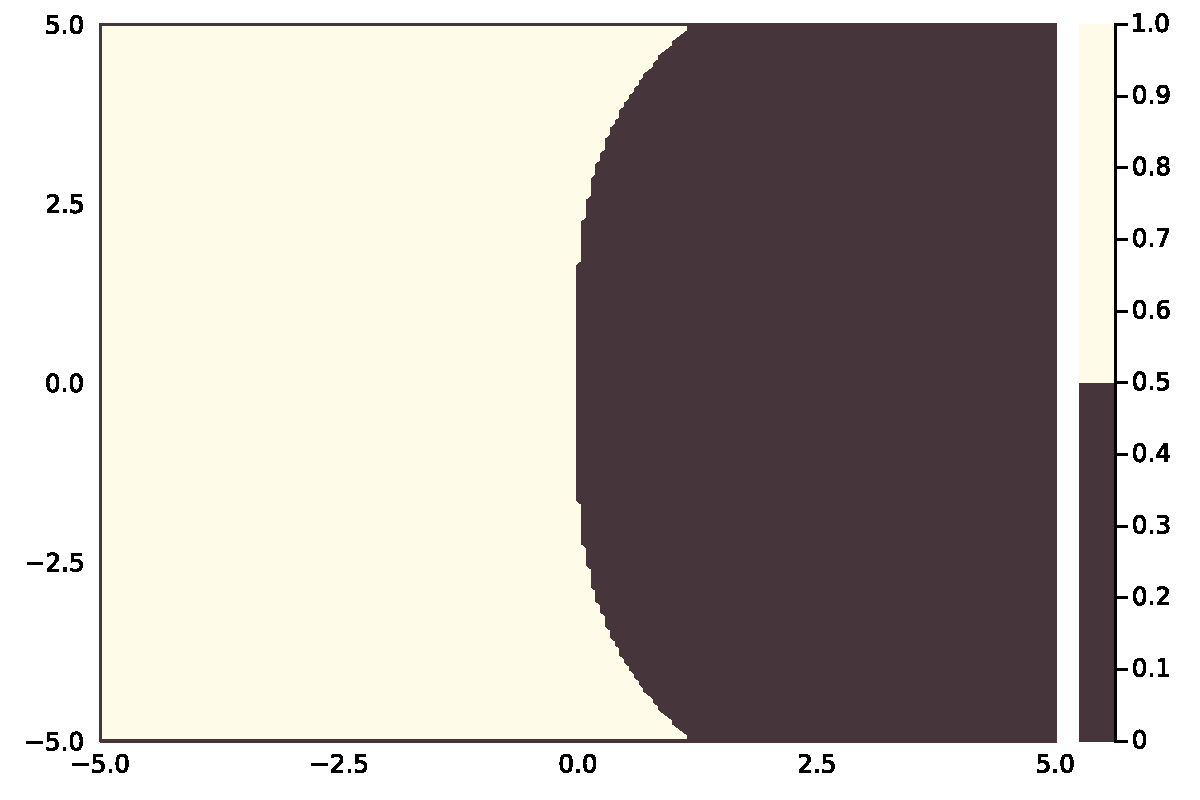
\includegraphics[width=\linewidth]{figures/ass_3_report_4_1.pdf}

\begin{lstlisting}
(*@\HLJLcs{{\#}}@*) (*@\HLJLcs{2s-DIRK}@*)
(*@\HLJLn{\ensuremath{\alpha}}@*) (*@\HLJLoB{=}@*) (*@\HLJLnfB{0.5}@*)
(*@\HLJLn{A}@*) (*@\HLJLoB{=}@*) (*@\HLJLp{[}@*)(*@\HLJLn{\ensuremath{\alpha}}@*) (*@\HLJLni{0}@*)
    (*@\HLJLni{1}@*)(*@\HLJLoB{-}@*)(*@\HLJLn{\ensuremath{\alpha}}@*) (*@\HLJLn{\ensuremath{\alpha}}@*)(*@\HLJLp{]}@*)
(*@\HLJLn{b}@*) (*@\HLJLoB{=}@*) (*@\HLJLp{[}@*)(*@\HLJLni{1}@*)(*@\HLJLoB{-}@*)(*@\HLJLn{\ensuremath{\alpha}}@*)(*@\HLJLp{,}@*) (*@\HLJLn{\ensuremath{\alpha}}@*)(*@\HLJLp{]}@*)

(*@\HLJLn{xs}@*)(*@\HLJLp{,}@*) (*@\HLJLn{Z}@*) (*@\HLJLoB{=}@*) (*@\HLJLnf{RASrk}@*)(*@\HLJLp{(}@*)(*@\HLJLn{A}@*)(*@\HLJLp{,}@*)(*@\HLJLn{b}@*)(*@\HLJLp{)}@*)
(*@\HLJLnf{contourf}@*)(*@\HLJLp{(}@*)(*@\HLJLn{xs}@*)(*@\HLJLp{,}@*)(*@\HLJLn{xs}@*)(*@\HLJLp{,}@*)(*@\HLJLn{Z}@*)(*@\HLJLp{,}@*) (*@\HLJLn{levels}@*) (*@\HLJLoB{=}@*) (*@\HLJLni{1}@*)(*@\HLJLp{)}@*)
\end{lstlisting}

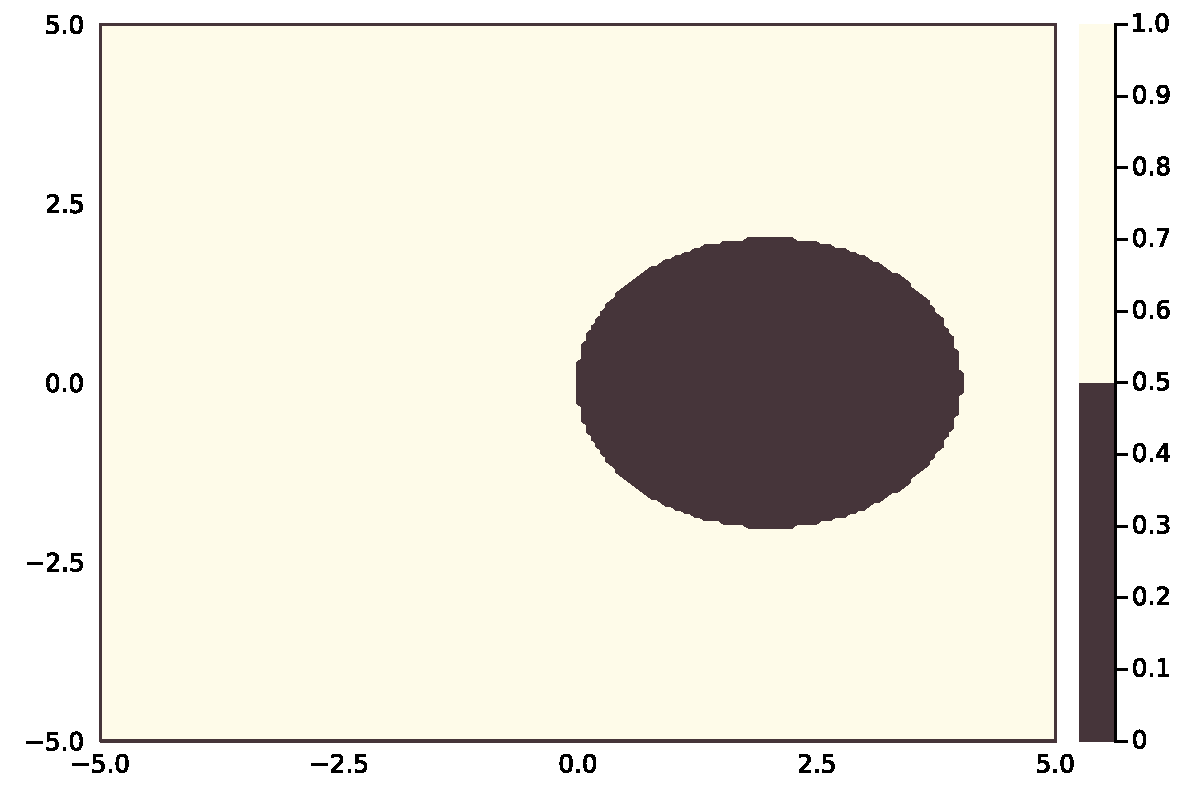
\includegraphics[width=\linewidth]{figures/ass_3_report_5_1.pdf}

\section{Problem 5}

\begin{lstlisting}
(*@\HLJLnf{f}@*)(*@\HLJLp{(}@*)(*@\HLJLn{u}@*)(*@\HLJLp{,}@*)(*@\HLJLn{t}@*)(*@\HLJLp{,}@*)(*@\HLJLn{\ensuremath{\mu}}@*)(*@\HLJLp{)}@*) (*@\HLJLoB{=}@*) (*@\HLJLoB{-}@*)(*@\HLJLp{(}@*)(*@\HLJLnfB{0.5}@*)(*@\HLJLoB{*}@*)(*@\HLJLnf{exp}@*)(*@\HLJLp{(}@*)(*@\HLJLni{20}@*)(*@\HLJLoB{*}@*)(*@\HLJLnf{cos}@*)(*@\HLJLp{(}@*)(*@\HLJLnfB{1.3}@*)(*@\HLJLoB{*}@*)(*@\HLJLn{t}@*)(*@\HLJLp{))}@*) (*@\HLJLoB{*}@*) (*@\HLJLnf{sinh}@*)(*@\HLJLp{(}@*)(*@\HLJLn{u}@*)(*@\HLJLoB{-}@*)(*@\HLJLnf{cos}@*)(*@\HLJLp{(}@*)(*@\HLJLn{t}@*)(*@\HLJLp{)));}@*)

(*@\HLJLn{\ensuremath{\alpha}}@*) (*@\HLJLoB{=}@*) (*@\HLJLni{1}@*) (*@\HLJLoB{-}@*) (*@\HLJLni{1}@*)(*@\HLJLoB{/}@*)(*@\HLJLnf{sqrt}@*)(*@\HLJLp{(}@*)(*@\HLJLni{2}@*)(*@\HLJLp{);}@*)
(*@\HLJLn{T}@*) (*@\HLJLoB{=}@*) (*@\HLJLnfB{30.0}@*)(*@\HLJLp{;}@*) (*@\HLJLn{h}@*) (*@\HLJLoB{=}@*) (*@\HLJLnfB{2.0}@*)(*@\HLJLoB{{\textasciicircum}}@*)(*@\HLJLp{(}@*)(*@\HLJLoB{-}@*)(*@\HLJLni{5}@*)(*@\HLJLp{);}@*) (*@\HLJLn{N}@*) (*@\HLJLoB{=}@*) (*@\HLJLnf{Int}@*)(*@\HLJLp{(}@*)(*@\HLJLn{T}@*)(*@\HLJLoB{/}@*)(*@\HLJLn{h}@*)(*@\HLJLp{);}@*)
(*@\HLJLn{u0}@*) (*@\HLJLoB{=}@*) (*@\HLJLnfB{0.0}@*)(*@\HLJLp{;}@*)

(*@\HLJLn{u}@*) (*@\HLJLoB{=}@*) (*@\HLJLnf{s2{\_}DIRK}@*)(*@\HLJLp{(}@*)(*@\HLJLn{f}@*)(*@\HLJLp{,}@*) (*@\HLJLn{N}@*)(*@\HLJLp{,}@*) (*@\HLJLn{T}@*)(*@\HLJLp{,}@*) (*@\HLJLn{u0}@*)(*@\HLJLp{,}@*) (*@\HLJLn{\ensuremath{\alpha}}@*)(*@\HLJLp{);}@*)
\end{lstlisting}


\subsection{Part 1}

\begin{lstlisting}
(*@\HLJLn{tList}@*) (*@\HLJLoB{=}@*) (*@\HLJLnf{collect}@*)(*@\HLJLp{(}@*)(*@\HLJLni{0}@*)(*@\HLJLoB{:}@*)(*@\HLJLn{N}@*)(*@\HLJLp{)}@*)(*@\HLJLoB{*}@*)(*@\HLJLp{(}@*)(*@\HLJLn{T}@*)(*@\HLJLoB{/}@*)(*@\HLJLn{N}@*)(*@\HLJLp{)}@*)
(*@\HLJLnf{plot}@*)(*@\HLJLp{(}@*)(*@\HLJLn{tList}@*)(*@\HLJLp{,}@*) (*@\HLJLn{u}@*)(*@\HLJLp{,}@*) (*@\HLJLn{label}@*) (*@\HLJLoB{=}@*) (*@\HLJLso{L"{}u(t)"{}}@*)(*@\HLJLp{,}@*) (*@\HLJLn{thickness{\_}scaling}@*) (*@\HLJLoB{=}@*)(*@\HLJLnfB{1.25}@*)(*@\HLJLp{)}@*)
(*@\HLJLnf{xlabel!}@*)(*@\HLJLp{(}@*)(*@\HLJLso{L"{}t"{}}@*)(*@\HLJLp{)}@*)
(*@\HLJLnf{ylabel!}@*)(*@\HLJLp{(}@*)(*@\HLJLso{L"{}u(t)"{}}@*)(*@\HLJLp{)}@*)
(*@\HLJLnf{title!}@*)(*@\HLJLp{(}@*)(*@\HLJLnf{latexstring}@*)(*@\HLJLp{(}@*)(*@\HLJLs{"{}2s-DIRK,h=2{\textasciicircum}{\{}-5{\}},T="{}}@*)(*@\HLJLp{,}@*)(*@\HLJLn{T}@*)(*@\HLJLp{))}@*)
(*@\HLJLnf{plot!}@*)(*@\HLJLp{(}@*)(*@\HLJLn{tList}@*)(*@\HLJLp{,}@*) (*@\HLJLn{cos}@*)(*@\HLJLoB{.}@*)(*@\HLJLp{(}@*)(*@\HLJLn{tList}@*)(*@\HLJLp{),}@*) (*@\HLJLn{label}@*) (*@\HLJLoB{=}@*) (*@\HLJLso{L"{}cos(t)"{}}@*)(*@\HLJLp{)}@*)
\end{lstlisting}

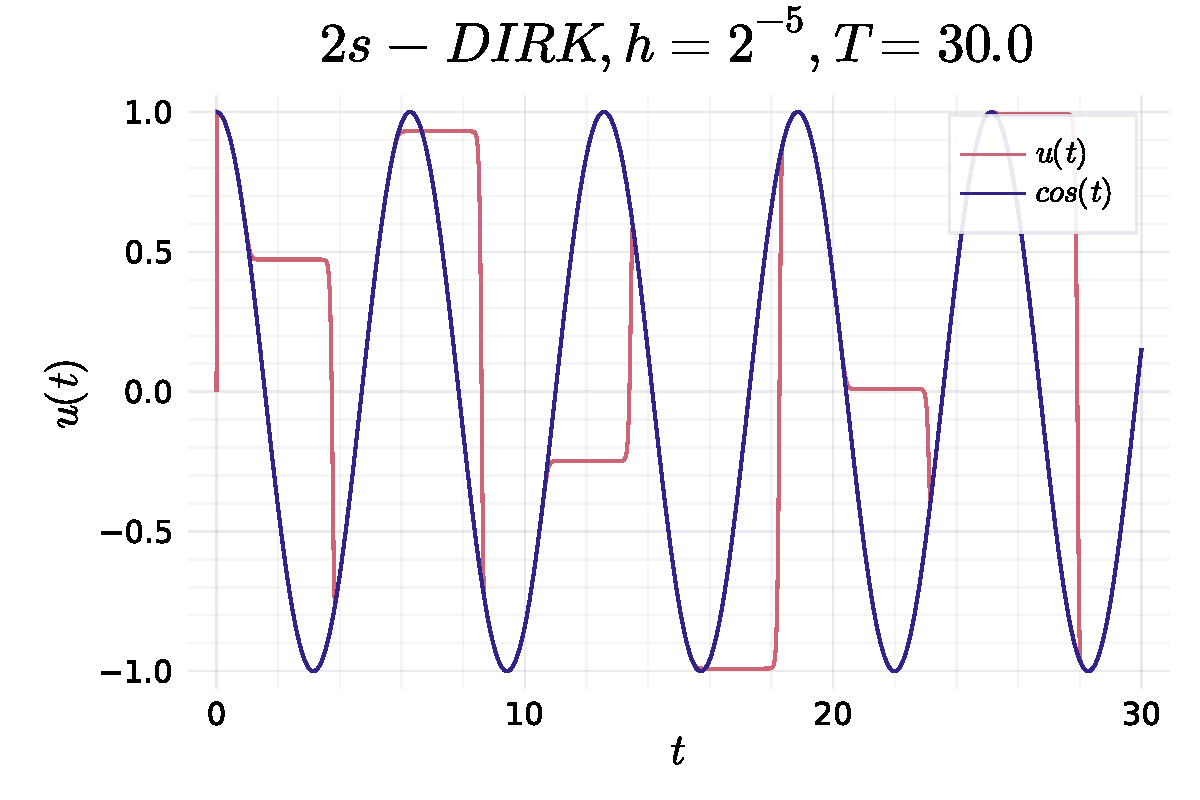
\includegraphics[width=\linewidth]{figures/ass_3_report_7_1.pdf}

\subsection{Part 2}

\begin{lstlisting}
(*@\HLJLnf{g}@*)(*@\HLJLp{(}@*)(*@\HLJLn{t}@*)(*@\HLJLp{)}@*) (*@\HLJLoB{=}@*) (*@\HLJLnfB{0.5}@*)(*@\HLJLoB{*}@*)(*@\HLJLnf{exp}@*)(*@\HLJLp{(}@*)(*@\HLJLni{20}@*)(*@\HLJLoB{*}@*)(*@\HLJLnf{cos}@*)(*@\HLJLp{(}@*)(*@\HLJLnfB{1.3}@*)(*@\HLJLoB{*}@*)(*@\HLJLn{t}@*)(*@\HLJLp{))}@*)
(*@\HLJLnf{plot}@*)(*@\HLJLp{(}@*)(*@\HLJLn{abs}@*)(*@\HLJLoB{.}@*)(*@\HLJLp{(}@*)(*@\HLJLn{u}@*) (*@\HLJLoB{-}@*) (*@\HLJLn{cos}@*)(*@\HLJLoB{.}@*)(*@\HLJLp{(}@*)(*@\HLJLn{tList}@*)(*@\HLJLp{)),}@*) (*@\HLJLn{g}@*)(*@\HLJLoB{.}@*)(*@\HLJLp{(}@*)(*@\HLJLn{tList}@*)(*@\HLJLp{),}@*) (*@\HLJLn{xaxis}@*)(*@\HLJLoB{=:}@*)(*@\HLJLn{log}@*)(*@\HLJLp{,}@*) (*@\HLJLn{yaxis}@*)(*@\HLJLoB{=:}@*)(*@\HLJLn{log}@*)(*@\HLJLp{,}@*) (*@\HLJLn{legend}@*) (*@\HLJLoB{=}@*) (*@\HLJLkc{false}@*)(*@\HLJLp{)}@*) 
(*@\HLJLnf{title!}@*)(*@\HLJLp{(}@*)(*@\HLJLs{"{}loglog}@*) (*@\HLJLs{plot"{}}@*)(*@\HLJLp{)}@*)
\end{lstlisting}

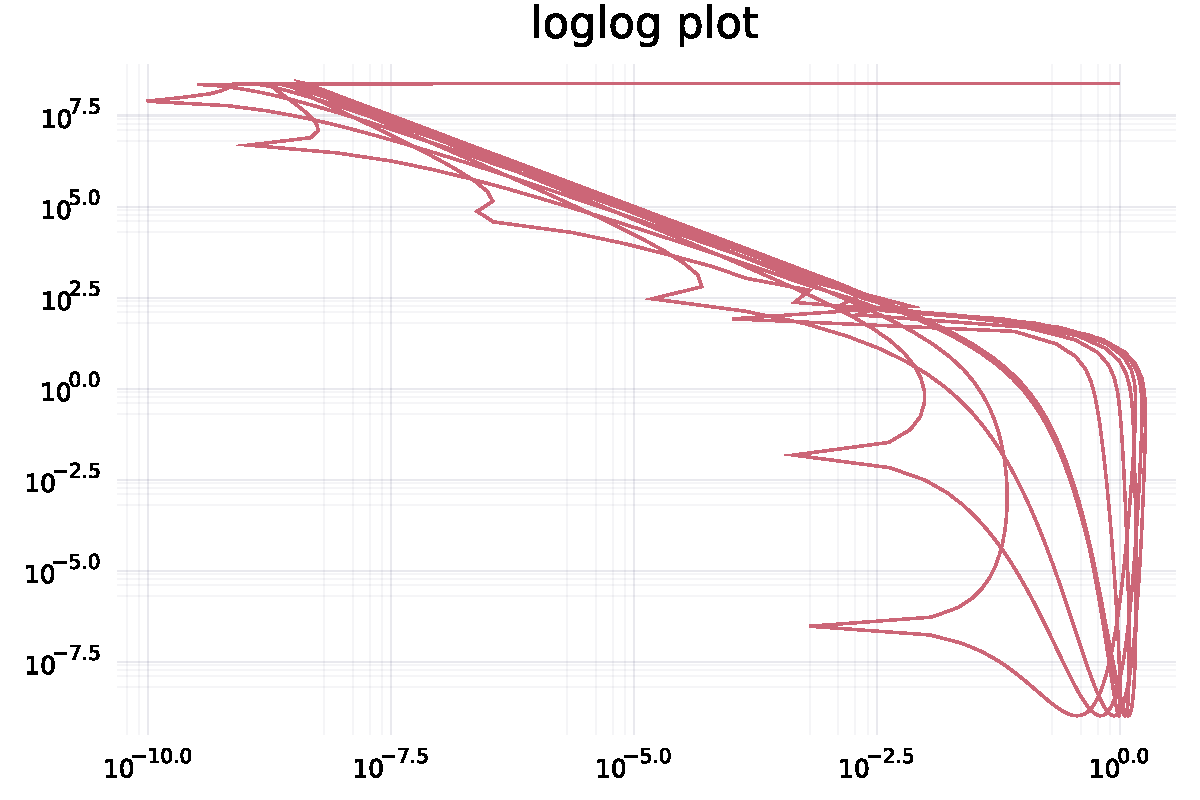
\includegraphics[width=\linewidth]{figures/ass_3_report_8_1.pdf}

\section{Problem 6}

\begin{lstlisting}
(*@\HLJLn{hs}@*) (*@\HLJLoB{=}@*) (*@\HLJLni{1}@*) (*@\HLJLoB{./}@*)(*@\HLJLp{(}@*)(*@\HLJLni{2}@*) (*@\HLJLoB{.{\textasciicircum}}@*)(*@\HLJLp{(}@*)(*@\HLJLni{3}@*)(*@\HLJLoB{:}@*)(*@\HLJLni{8}@*)(*@\HLJLp{))}@*)
(*@\HLJLk{for}@*) (*@\HLJLn{i}@*) (*@\HLJLoB{=}@*) (*@\HLJLni{1}@*) (*@\HLJLoB{:}@*) (*@\HLJLnf{length}@*)(*@\HLJLp{(}@*)(*@\HLJLn{hs}@*)(*@\HLJLp{)}@*)
    (*@\HLJLn{N}@*) (*@\HLJLoB{=}@*) (*@\HLJLnf{Int}@*)(*@\HLJLp{(}@*)(*@\HLJLn{T}@*)(*@\HLJLoB{/}@*)(*@\HLJLn{hs}@*)(*@\HLJLp{[}@*)(*@\HLJLn{i}@*)(*@\HLJLp{])}@*)
    (*@\HLJLn{tList}@*) (*@\HLJLoB{=}@*) (*@\HLJLnf{collect}@*)(*@\HLJLp{(}@*)(*@\HLJLni{0}@*)(*@\HLJLoB{:}@*)(*@\HLJLn{N}@*)(*@\HLJLp{)}@*)(*@\HLJLoB{*}@*)(*@\HLJLp{(}@*)(*@\HLJLn{T}@*)(*@\HLJLoB{/}@*)(*@\HLJLn{N}@*)(*@\HLJLp{)}@*)

    (*@\HLJLcs{{\#}{\#}}@*) (*@\HLJLcs{Backward}@*) (*@\HLJLcs{Euler}@*)
    (*@\HLJLn{u{\_}euler}@*) (*@\HLJLoB{=}@*) (*@\HLJLnf{BackwardEuler{\_}n}@*)(*@\HLJLp{(}@*)(*@\HLJLn{f}@*)(*@\HLJLp{,}@*) (*@\HLJLn{N}@*)(*@\HLJLp{,}@*) (*@\HLJLn{T}@*)(*@\HLJLp{,}@*) (*@\HLJLn{u0}@*)(*@\HLJLp{)}@*)
    (*@\HLJLn{u{\_}eexact}@*) (*@\HLJLoB{=}@*) (*@\HLJLnf{BackwardEuler{\_}n}@*)(*@\HLJLp{(}@*)(*@\HLJLn{f}@*)(*@\HLJLp{,}@*)(*@\HLJLni{2}@*)(*@\HLJLoB{*}@*)(*@\HLJLn{N}@*)(*@\HLJLp{,}@*)(*@\HLJLn{T}@*)(*@\HLJLp{,}@*)(*@\HLJLn{u0}@*)(*@\HLJLp{)}@*)
    (*@\HLJLn{euler{\_}error}@*) (*@\HLJLoB{=}@*) (*@\HLJLn{abs}@*)(*@\HLJLoB{.}@*)(*@\HLJLp{(}@*)(*@\HLJLn{u{\_}euler}@*)(*@\HLJLp{[}@*)(*@\HLJLni{1}@*)(*@\HLJLoB{:}@*)(*@\HLJLn{N}@*)(*@\HLJLp{]}@*) (*@\HLJLoB{-}@*) (*@\HLJLn{u{\_}eexact}@*)(*@\HLJLp{[}@*)(*@\HLJLni{1}@*)(*@\HLJLoB{:}@*)(*@\HLJLni{2}@*)(*@\HLJLoB{:}@*)(*@\HLJLni{2}@*)(*@\HLJLoB{*}@*)(*@\HLJLn{N}@*)(*@\HLJLp{])}@*)(*@\HLJLoB{./}@*)(*@\HLJLp{(}@*)(*@\HLJLni{1}@*)(*@\HLJLoB{-}@*)(*@\HLJLnfB{0.5}@*)(*@\HLJLoB{{\textasciicircum}}@*)(*@\HLJLni{1}@*)(*@\HLJLp{)}@*) (*@\HLJLcs{{\#}}@*) (*@\HLJLcs{first}@*) (*@\HLJLcs{order}@*) (*@\HLJLcs{method}@*)
    (*@\HLJLn{p1}@*) (*@\HLJLoB{=}@*) (*@\HLJLnf{plot}@*)(*@\HLJLp{(}@*)(*@\HLJLn{tList}@*)(*@\HLJLp{[}@*)(*@\HLJLni{2}@*)(*@\HLJLoB{:}@*)(*@\HLJLn{N}@*)(*@\HLJLp{],}@*) (*@\HLJLn{euler{\_}error}@*)(*@\HLJLp{[}@*)(*@\HLJLni{2}@*)(*@\HLJLoB{:}@*)(*@\HLJLn{N}@*)(*@\HLJLp{],}@*) (*@\HLJLn{label}@*) (*@\HLJLoB{=}@*) (*@\HLJLs{"{}Backward}@*) (*@\HLJLs{Euler"{}}@*)(*@\HLJLp{,}@*) (*@\HLJLn{xaxis}@*)(*@\HLJLoB{=:}@*)(*@\HLJLn{log}@*)(*@\HLJLp{,}@*) (*@\HLJLn{yaxis}@*)(*@\HLJLoB{=:}@*)(*@\HLJLn{log}@*)(*@\HLJLp{,}@*) (*@\HLJLn{marker}@*) (*@\HLJLoB{=}@*) (*@\HLJLp{(}@*)(*@\HLJLsc{:square}@*)(*@\HLJLp{,}@*)(*@\HLJLni{5}@*)(*@\HLJLp{))}@*)
    (*@\HLJLnf{xaxis!}@*)(*@\HLJLp{(}@*)(*@\HLJLso{L"{}t"{}}@*)(*@\HLJLp{)}@*)
    (*@\HLJLnf{yaxis!}@*)(*@\HLJLp{(}@*)(*@\HLJLso{L"{}u(t)"{}}@*)(*@\HLJLp{)}@*)
    (*@\HLJLnf{title!}@*)(*@\HLJLp{(}@*)(*@\HLJLnf{latexstring}@*)(*@\HLJLp{(}@*)(*@\HLJLs{"{}Error}@*) (*@\HLJLs{Estimate,h="{}}@*)(*@\HLJLp{,}@*)(*@\HLJLn{hs}@*)(*@\HLJLp{[}@*)(*@\HLJLn{i}@*)(*@\HLJLp{]))}@*)

    (*@\HLJLcs{{\#}{\#}}@*) (*@\HLJLcs{s2-DIRK}@*)
    (*@\HLJLn{u{\_}s2{\_}DIRK}@*) (*@\HLJLoB{=}@*) (*@\HLJLnf{s2{\_}DIRK}@*)(*@\HLJLp{(}@*)(*@\HLJLn{f}@*)(*@\HLJLp{,}@*) (*@\HLJLn{N}@*)(*@\HLJLp{,}@*) (*@\HLJLn{T}@*)(*@\HLJLp{,}@*) (*@\HLJLn{u0}@*)(*@\HLJLp{,}@*) (*@\HLJLn{\ensuremath{\alpha}}@*)(*@\HLJLp{)}@*)
    (*@\HLJLn{u{\_}Dexact}@*) (*@\HLJLoB{=}@*) (*@\HLJLnf{s2{\_}DIRK}@*)(*@\HLJLp{(}@*)(*@\HLJLn{f}@*)(*@\HLJLp{,}@*) (*@\HLJLni{2}@*)(*@\HLJLoB{*}@*)(*@\HLJLn{N}@*)(*@\HLJLp{,}@*) (*@\HLJLn{T}@*)(*@\HLJLp{,}@*) (*@\HLJLn{u0}@*)(*@\HLJLp{,}@*) (*@\HLJLn{\ensuremath{\alpha}}@*)(*@\HLJLp{)}@*)
    (*@\HLJLn{DIRK{\_}error}@*) (*@\HLJLoB{=}@*) (*@\HLJLn{abs}@*)(*@\HLJLoB{.}@*)(*@\HLJLp{(}@*)(*@\HLJLn{u{\_}s2{\_}DIRK}@*)(*@\HLJLp{[}@*)(*@\HLJLni{1}@*)(*@\HLJLoB{:}@*)(*@\HLJLn{N}@*)(*@\HLJLp{]}@*) (*@\HLJLoB{-}@*) (*@\HLJLn{u{\_}Dexact}@*)(*@\HLJLp{[}@*)(*@\HLJLni{1}@*)(*@\HLJLoB{:}@*)(*@\HLJLni{2}@*)(*@\HLJLoB{:}@*)(*@\HLJLni{2}@*)(*@\HLJLoB{*}@*)(*@\HLJLn{N}@*)(*@\HLJLp{])}@*)(*@\HLJLoB{./}@*)(*@\HLJLp{(}@*)(*@\HLJLni{1}@*)(*@\HLJLoB{-}@*)(*@\HLJLnfB{0.5}@*)(*@\HLJLoB{{\textasciicircum}}@*)(*@\HLJLni{2}@*)(*@\HLJLp{)}@*) (*@\HLJLcs{{\#}}@*) (*@\HLJLcs{second}@*) (*@\HLJLcs{order}@*) (*@\HLJLcs{method}@*)
    (*@\HLJLn{p2}@*) (*@\HLJLoB{=}@*) (*@\HLJLnf{plot!}@*)(*@\HLJLp{(}@*)(*@\HLJLn{tList}@*)(*@\HLJLp{[}@*)(*@\HLJLni{2}@*)(*@\HLJLoB{:}@*)(*@\HLJLn{N}@*)(*@\HLJLp{],}@*) (*@\HLJLn{DIRK{\_}error}@*)(*@\HLJLp{[}@*)(*@\HLJLni{2}@*)(*@\HLJLoB{:}@*)(*@\HLJLn{N}@*)(*@\HLJLp{],}@*) (*@\HLJLn{label}@*) (*@\HLJLoB{=}@*) (*@\HLJLs{"{}2s-DIRK}@*) (*@\HLJLs{error"{}}@*)(*@\HLJLp{,}@*) (*@\HLJLn{xaxis}@*)(*@\HLJLoB{=:}@*)(*@\HLJLn{log}@*)(*@\HLJLp{,}@*) (*@\HLJLn{yaxis}@*)(*@\HLJLoB{=:}@*)(*@\HLJLn{log}@*)(*@\HLJLp{,}@*) (*@\HLJLn{marker}@*) (*@\HLJLoB{=}@*) (*@\HLJLp{(}@*)(*@\HLJLsc{:square}@*)(*@\HLJLp{,}@*)(*@\HLJLni{5}@*)(*@\HLJLp{))}@*)
    (*@\HLJLnf{display}@*)(*@\HLJLp{(}@*)(*@\HLJLn{p2}@*)(*@\HLJLp{)}@*)
(*@\HLJLk{end}@*)
\end{lstlisting}

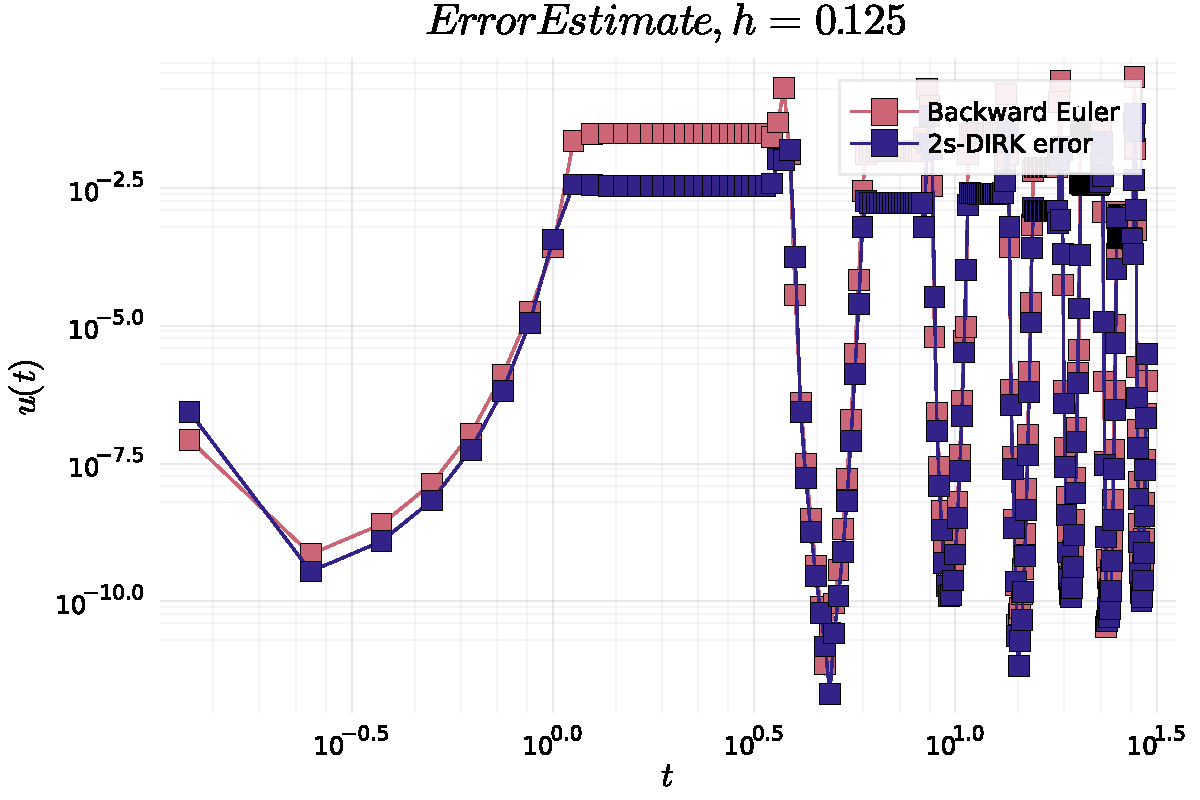
\includegraphics[width=\linewidth]{figures/ass_3_report_9_1.pdf}
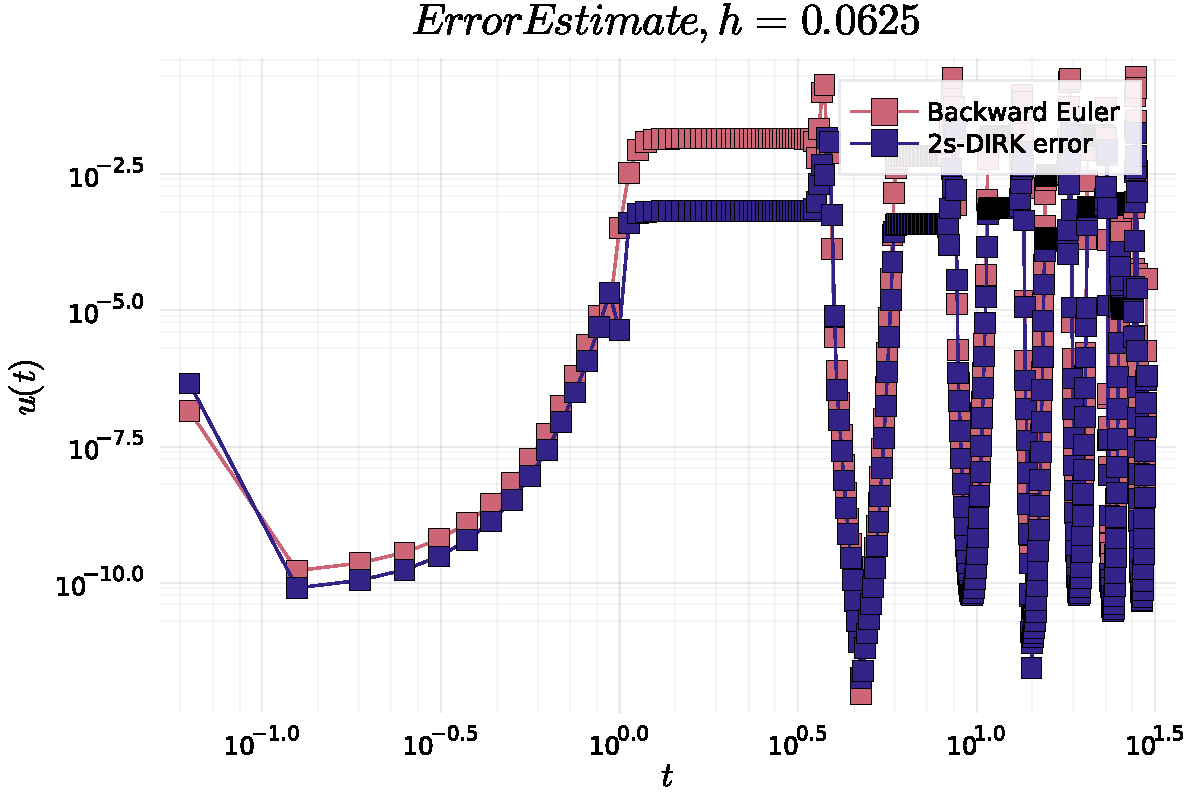
\includegraphics[width=\linewidth]{figures/ass_3_report_9_2.pdf}
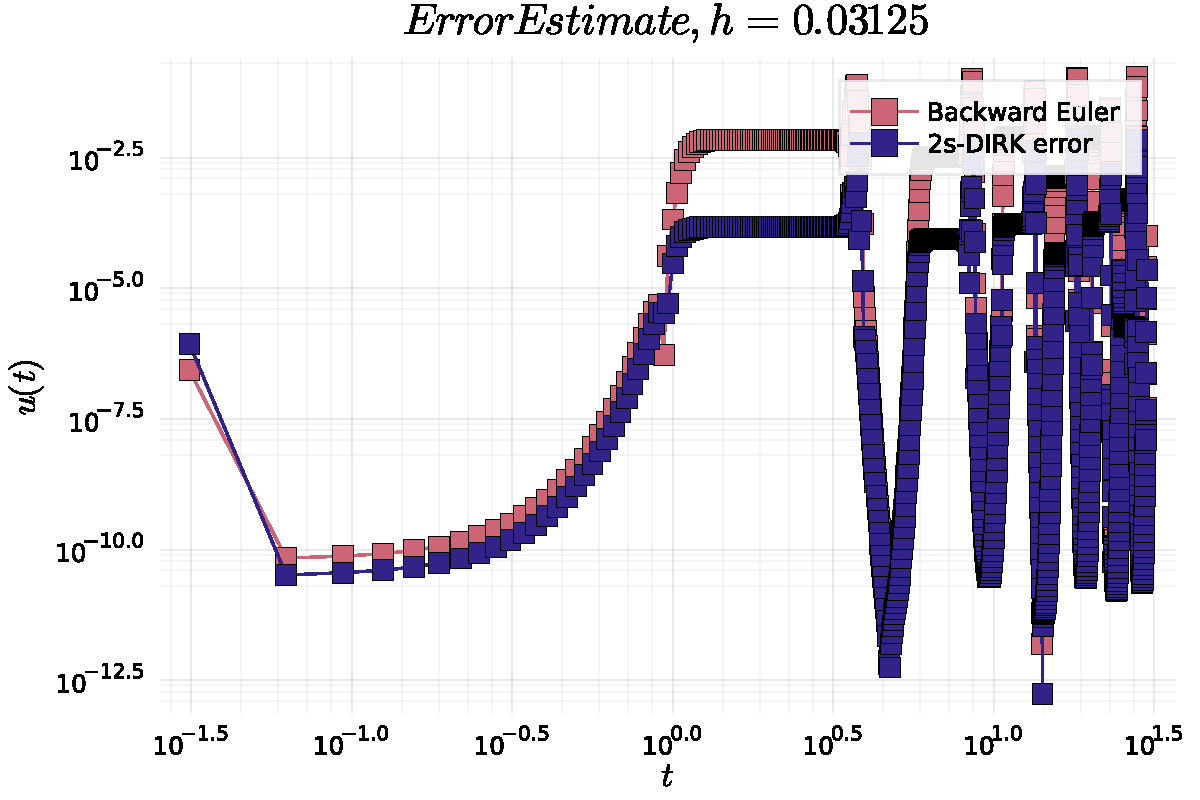
\includegraphics[width=\linewidth]{figures/ass_3_report_9_3.pdf}
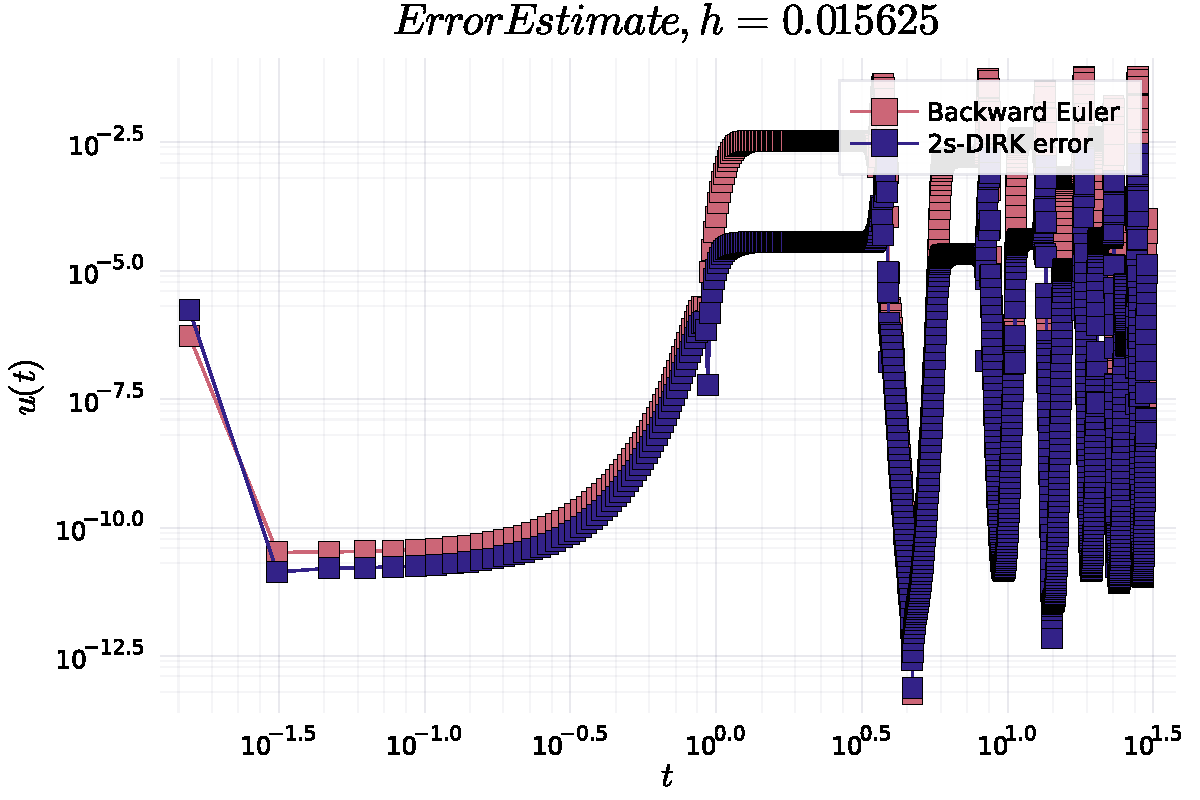
\includegraphics[width=\linewidth]{figures/ass_3_report_9_4.pdf}
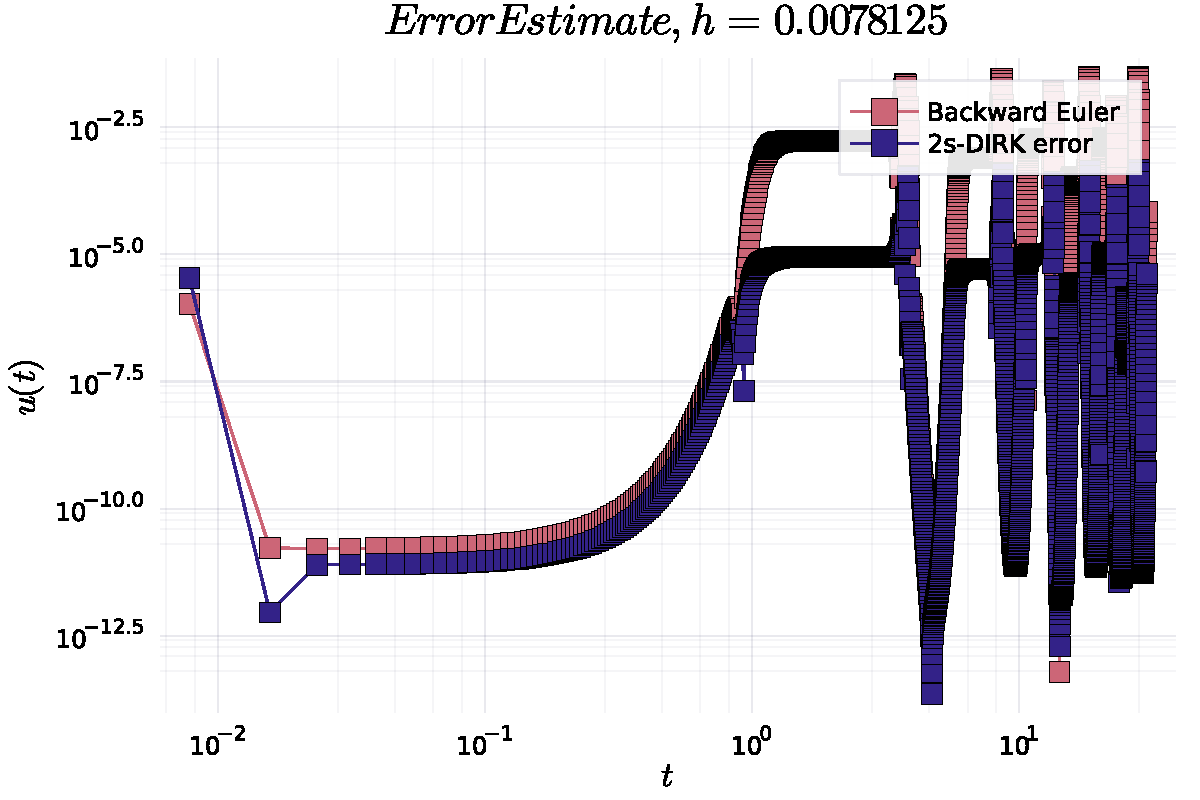
\includegraphics[width=\linewidth]{figures/ass_3_report_9_5.pdf}
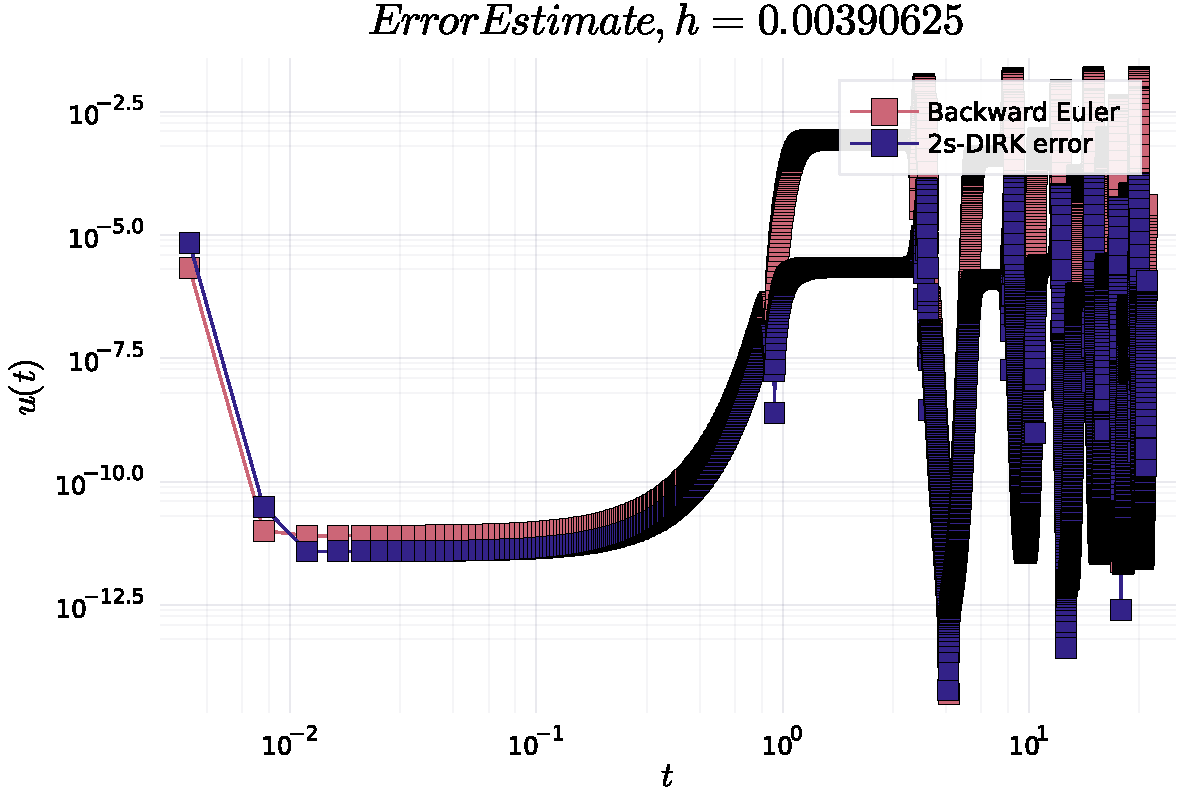
\includegraphics[width=\linewidth]{figures/ass_3_report_9_6.pdf}

\subsubsection{Part 2}

\begin{lstlisting}
(*@\HLJLn{h}@*) (*@\HLJLoB{=}@*) (*@\HLJLnfB{2.0}@*)(*@\HLJLoB{{\textasciicircum}}@*)(*@\HLJLp{(}@*)(*@\HLJLoB{-}@*)(*@\HLJLni{7}@*)(*@\HLJLp{)}@*)
(*@\HLJLn{N}@*) (*@\HLJLoB{=}@*) (*@\HLJLnf{Int}@*)(*@\HLJLp{(}@*)(*@\HLJLn{T}@*)(*@\HLJLoB{/}@*)(*@\HLJLn{h}@*)(*@\HLJLp{)}@*)
(*@\HLJLn{tList}@*) (*@\HLJLoB{=}@*) (*@\HLJLnf{collect}@*)(*@\HLJLp{(}@*)(*@\HLJLni{0}@*)(*@\HLJLoB{:}@*)(*@\HLJLn{N}@*)(*@\HLJLp{)}@*)(*@\HLJLoB{*}@*)(*@\HLJLp{(}@*)(*@\HLJLn{T}@*)(*@\HLJLoB{/}@*)(*@\HLJLn{N}@*)(*@\HLJLp{)}@*)

(*@\HLJLcs{{\#}{\#}}@*) (*@\HLJLcs{Backward}@*) (*@\HLJLcs{Euler}@*)
(*@\HLJLn{u{\_}euler}@*) (*@\HLJLoB{=}@*) (*@\HLJLnf{BackwardEuler{\_}n}@*)(*@\HLJLp{(}@*)(*@\HLJLn{f}@*)(*@\HLJLp{,}@*) (*@\HLJLn{N}@*)(*@\HLJLp{,}@*) (*@\HLJLn{T}@*)(*@\HLJLp{,}@*) (*@\HLJLn{u0}@*)(*@\HLJLp{)}@*)
(*@\HLJLn{u{\_}eexact}@*) (*@\HLJLoB{=}@*) (*@\HLJLnf{BackwardEuler{\_}n}@*)(*@\HLJLp{(}@*)(*@\HLJLn{f}@*)(*@\HLJLp{,}@*)(*@\HLJLni{2}@*)(*@\HLJLoB{*}@*)(*@\HLJLn{N}@*)(*@\HLJLp{,}@*)(*@\HLJLn{T}@*)(*@\HLJLp{,}@*)(*@\HLJLn{u0}@*)(*@\HLJLp{)}@*)
(*@\HLJLn{euler{\_}error}@*) (*@\HLJLoB{=}@*) (*@\HLJLn{abs}@*)(*@\HLJLoB{.}@*)(*@\HLJLp{(}@*)(*@\HLJLn{u{\_}euler}@*)(*@\HLJLp{[}@*)(*@\HLJLni{1}@*)(*@\HLJLoB{:}@*)(*@\HLJLn{N}@*)(*@\HLJLp{]}@*) (*@\HLJLoB{-}@*) (*@\HLJLn{u{\_}eexact}@*)(*@\HLJLp{[}@*)(*@\HLJLni{1}@*)(*@\HLJLoB{:}@*)(*@\HLJLni{2}@*)(*@\HLJLoB{:}@*)(*@\HLJLni{2}@*)(*@\HLJLoB{*}@*)(*@\HLJLn{N}@*)(*@\HLJLp{])}@*)(*@\HLJLoB{./}@*)(*@\HLJLp{(}@*)(*@\HLJLni{1}@*)(*@\HLJLoB{-}@*)(*@\HLJLnfB{0.5}@*)(*@\HLJLoB{{\textasciicircum}}@*)(*@\HLJLni{1}@*)(*@\HLJLp{)}@*) (*@\HLJLcs{{\#}}@*) (*@\HLJLcs{first}@*) (*@\HLJLcs{order}@*) (*@\HLJLcs{method}@*)
(*@\HLJLn{p1}@*) (*@\HLJLoB{=}@*) (*@\HLJLnf{plot}@*)(*@\HLJLp{(}@*)(*@\HLJLn{tList}@*)(*@\HLJLp{[}@*)(*@\HLJLni{2}@*)(*@\HLJLoB{:}@*)(*@\HLJLn{N}@*)(*@\HLJLp{],}@*) (*@\HLJLn{euler{\_}error}@*)(*@\HLJLp{[}@*)(*@\HLJLni{2}@*)(*@\HLJLoB{:}@*)(*@\HLJLn{N}@*)(*@\HLJLp{],}@*) (*@\HLJLn{label}@*) (*@\HLJLoB{=}@*) (*@\HLJLs{"{}Backward}@*) (*@\HLJLs{Euler"{}}@*)(*@\HLJLp{,}@*) (*@\HLJLn{xaxis}@*)(*@\HLJLoB{=:}@*)(*@\HLJLn{log}@*)(*@\HLJLp{,}@*) (*@\HLJLn{yaxis}@*)(*@\HLJLoB{=:}@*)(*@\HLJLn{log}@*)(*@\HLJLp{,}@*) (*@\HLJLn{marker}@*) (*@\HLJLoB{=}@*) (*@\HLJLp{(}@*)(*@\HLJLsc{:square}@*)(*@\HLJLp{,}@*)(*@\HLJLni{5}@*)(*@\HLJLp{))}@*)
(*@\HLJLnf{xaxis!}@*)(*@\HLJLp{(}@*)(*@\HLJLso{L"{}t"{}}@*)(*@\HLJLp{)}@*)
(*@\HLJLnf{yaxis!}@*)(*@\HLJLp{(}@*)(*@\HLJLso{L"{}u(t)"{}}@*)(*@\HLJLp{)}@*)
(*@\HLJLnf{title!}@*)(*@\HLJLp{(}@*)(*@\HLJLnf{latexstring}@*)(*@\HLJLp{(}@*)(*@\HLJLs{"{}Error}@*) (*@\HLJLs{Estimate,h="{}}@*)(*@\HLJLp{,}@*)(*@\HLJLn{h}@*)(*@\HLJLp{))}@*)

(*@\HLJLcs{{\#}{\#}}@*) (*@\HLJLcs{s2-DIRK}@*)
(*@\HLJLn{u{\_}s2{\_}DIRK}@*) (*@\HLJLoB{=}@*) (*@\HLJLnf{s2{\_}DIRK}@*)(*@\HLJLp{(}@*)(*@\HLJLn{f}@*)(*@\HLJLp{,}@*) (*@\HLJLn{N}@*)(*@\HLJLp{,}@*) (*@\HLJLn{T}@*)(*@\HLJLp{,}@*) (*@\HLJLn{u0}@*)(*@\HLJLp{,}@*) (*@\HLJLn{\ensuremath{\alpha}}@*)(*@\HLJLp{)}@*)
(*@\HLJLn{u{\_}Dexact}@*) (*@\HLJLoB{=}@*) (*@\HLJLnf{s2{\_}DIRK}@*)(*@\HLJLp{(}@*)(*@\HLJLn{f}@*)(*@\HLJLp{,}@*) (*@\HLJLni{2}@*)(*@\HLJLoB{*}@*)(*@\HLJLn{N}@*)(*@\HLJLp{,}@*) (*@\HLJLn{T}@*)(*@\HLJLp{,}@*) (*@\HLJLn{u0}@*)(*@\HLJLp{,}@*) (*@\HLJLn{\ensuremath{\alpha}}@*)(*@\HLJLp{)}@*)
(*@\HLJLn{DIRK{\_}error}@*) (*@\HLJLoB{=}@*) (*@\HLJLn{abs}@*)(*@\HLJLoB{.}@*)(*@\HLJLp{(}@*)(*@\HLJLn{u{\_}s2{\_}DIRK}@*)(*@\HLJLp{[}@*)(*@\HLJLni{1}@*)(*@\HLJLoB{:}@*)(*@\HLJLn{N}@*)(*@\HLJLp{]}@*) (*@\HLJLoB{-}@*) (*@\HLJLn{u{\_}Dexact}@*)(*@\HLJLp{[}@*)(*@\HLJLni{1}@*)(*@\HLJLoB{:}@*)(*@\HLJLni{2}@*)(*@\HLJLoB{:}@*)(*@\HLJLni{2}@*)(*@\HLJLoB{*}@*)(*@\HLJLn{N}@*)(*@\HLJLp{])}@*)(*@\HLJLoB{./}@*)(*@\HLJLp{(}@*)(*@\HLJLni{1}@*)(*@\HLJLoB{-}@*)(*@\HLJLnfB{0.5}@*)(*@\HLJLoB{{\textasciicircum}}@*)(*@\HLJLni{2}@*)(*@\HLJLp{)}@*) (*@\HLJLcs{{\#}}@*) (*@\HLJLcs{second}@*) (*@\HLJLcs{order}@*) (*@\HLJLcs{method}@*)
(*@\HLJLn{p2}@*) (*@\HLJLoB{=}@*) (*@\HLJLnf{plot!}@*)(*@\HLJLp{(}@*)(*@\HLJLn{tList}@*)(*@\HLJLp{[}@*)(*@\HLJLni{2}@*)(*@\HLJLoB{:}@*)(*@\HLJLn{N}@*)(*@\HLJLp{],}@*) (*@\HLJLn{DIRK{\_}error}@*)(*@\HLJLp{[}@*)(*@\HLJLni{2}@*)(*@\HLJLoB{:}@*)(*@\HLJLn{N}@*)(*@\HLJLp{],}@*) (*@\HLJLn{label}@*) (*@\HLJLoB{=}@*) (*@\HLJLs{"{}2s-DIRK}@*) (*@\HLJLs{error"{}}@*)(*@\HLJLp{,}@*) (*@\HLJLn{xaxis}@*)(*@\HLJLoB{=:}@*)(*@\HLJLn{log}@*)(*@\HLJLp{,}@*) (*@\HLJLn{yaxis}@*)(*@\HLJLoB{=:}@*)(*@\HLJLn{log}@*)(*@\HLJLp{,}@*) (*@\HLJLn{marker}@*) (*@\HLJLoB{=}@*) (*@\HLJLp{(}@*)(*@\HLJLsc{:square}@*)(*@\HLJLp{,}@*)(*@\HLJLni{5}@*)(*@\HLJLp{))}@*)
(*@\HLJLnf{display}@*)(*@\HLJLp{(}@*)(*@\HLJLn{p2}@*)(*@\HLJLp{)}@*)
\end{lstlisting}

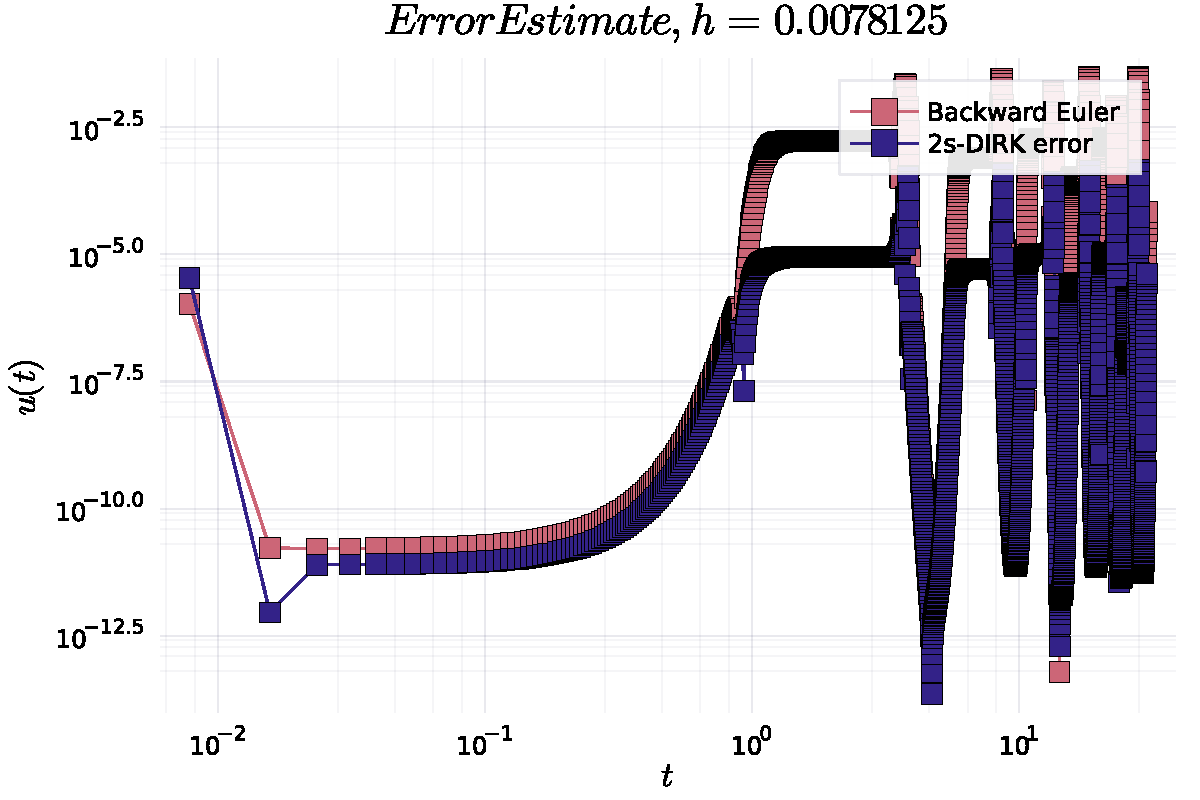
\includegraphics[width=\linewidth]{figures/ass_3_report_10_1.pdf}


\end{document}
